%_____________________________________________________________________________________________
% Department of Comp/IT BTech Project Report
%_____________________________________________________________________________________________

\chapter{System Design}

  \section{Architecture overview}
  A multi-step process will be followed to convert the images provided by the user into a functional code. The process is broadly divided into two steps:
  \begin{itemize}
		\item Processing images to detect and label ROI and storing in  a structured format.
    \item Conversion of structured specification of ROI into target code.
	\end{itemize}
  Initially a different approach was experimented which was a single step process. This was heavily relying on the neural networks’ training and accuracy. But it was observed that the dataset available for training was not adequate and using such a complex neural network was an overkill as the problem at hand can be categorized as a image classification problem. Hence an improved architecture was used to implement the solution
  \begin{figure}
		\centering
		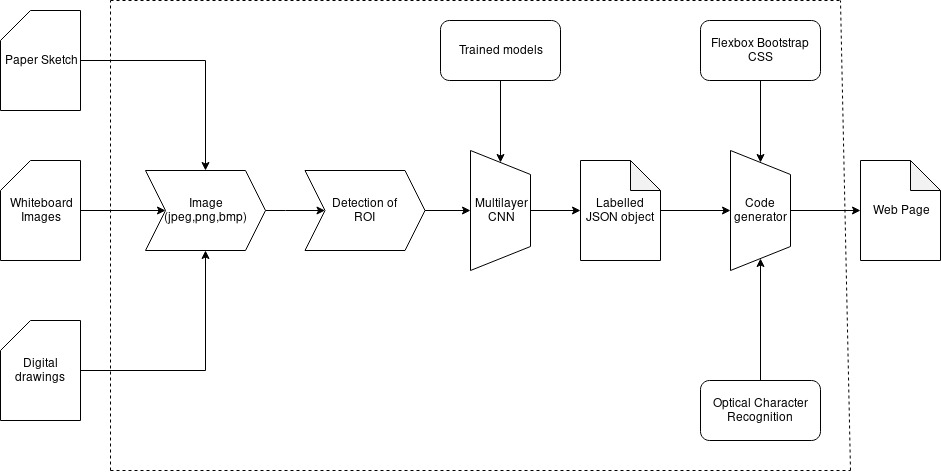
\includegraphics[width=6in]{architecture}
		\caption
		{A block diagram of the complete process}
	\end{figure}

  \section{Vision Model}
    An integral part of our solution is to understand the mock up sketch image the user provides. We need a solution to detect the regions of interests (ROIs) from the user provided hand drawn sketch, identify the DOM element corresponding to the drawing, and detect handwritten texts within the sketch. The advancements in image processing and computer vision provides many possible methods to do the same. We have different classification and detection model architectures available to work with which are proven to give better results. Also some image preprocessing and dataset augmentation methods can boost the results of these models. We will discuss the experiments performed and the method we used for our solution.

    \subsection{Experiments with Object Detection Algorithms}
      Object Detection Algorithms are different from classification algorithms. The difference between object detection algorithms and classification algorithms is that in detection algorithms, we try to draw a bounding box around the object of interest to locate it within the image. Unlike image classification, this problem cannot be solved by building a standard convolutional network followed by a fully connected layer. The reason being that the output layer here is not constant and variable in size, because the image can have variable number of occurence of objects in an image. Therefore, a different set of algorithms like R-CNN [8], Faster-RCNN [9] and YOLO [10] are used which are helpful in solving the problem of finding and classifying design layout elements[1]. These networks are capable of finding the ROIs as well as classifying them into classes.

    \subsection{RCNN}
      The RCNN uses selective search to find out the region proposals. Using this algorithm around 2000 regions are detected. The regions are of various sizes and aspect ratio spread over the image depending on the image features and contours defined in the selective search algorithm. These proposed regions are then passed to a Convolutional Neural Network for classification and elimination.
      Selective search combined with a simple CNN was used to implement this method. The CNN classification accuracy was around 81%. But the main challenge was elimination of hierarchical regions (regions inside regions). Therefore many regions were detected in a same image.
      The speed of RCNN is slow and was difficult to use it for a real time application. Moreover the model trained on the available training data generated a lot of false ROIs and gave poor results. With the help of more diverse training a data a better model could have been trained. But however the speed of RCNN is always an issue for real time implementation.

    \subsection{YOLO (You Only Look Once)}
      YOLO as the name suggests looks at the image only once. In this architecture there is no separate model for region proposals. The output of the network is regions along with its class. It also makes predictions with a single network evaluation unlike systems like R-CNN which require thousands for a single image. This makes it extremely fast, more than 1000x faster than R-CNN and 100x faster than Fast R-CNN.
      YOLO and such models require a large training dataset and are very particular and fitting our dataset to this model was difficult. It was difficult to find a configuration for which the model was at least able to overfit on the dataset. The difficulty in finding the configuration and very less dataset even to overfit was the reason further experiment on this model was stopped.

    \subsection{Faster-RCNN}
      Selective search is a slow and time-consuming process affecting the performance of the network. Therefore, Faster RCNN uses an object detection algorithm that eliminates the selective search algorithm and lets the network learn the region proposals. These networks are called Region Proposals Networks (RPNs). The image is provided as an input to a convolutional network which provides a convolutional feature map. The predicted region proposals are then reshaped using a RoI pooling layer which is then used to classify the image within the proposed region and predict the offset values for the bounding boxes.
      Faster-RCNN model proved better than both RCNN and YOLO. The classification accuracy was around 82% but it was short on finding all the ROIs. The RPN loss was unable to decrease after a certain point. As a result not all the ROIs were detected in an image; which is a major drawback in our application. It leads to missing out some DOM elements. Better results through separate detection and classification method and unavailability of big and diverse dataset held us from experimenting further with this network.

    \subsection{Conclusion}
      The above models were tried to train on a dataset containing of around 100 labelled images. With the experiments performed to train these complex algorithms; it was clearly observed that more training data and diverse data was required.
      Some data augmentation techniques like binarizing the image, changing color values and changing contrast values were applied on the available images. Other augmentation techniques like flipping and rotating the images were not applicable for the problem set.
      The techniques did not increase the dataset significantly and the only option seemed to be creating more hand-drawn design layout images and manually labelling all the DOM elements in it.

  \section{Modified Approach}
    The input image provided by the user is usually of two colors : the ink and the background colors. These high contrast of colors can be used to detect regions first and then later classify them. Also the above models performed poorly on the ROI detection phase and not the classification phase. The image pre-processing can be done using tools like OpenCV to get the desired regions.
    The results conspicuously hinted towards another approach by finding the Regions and Interests first, rather than Object Detection over the whole image, and then using modified deep learning algorithms to identify the DOM elements.
    So the task of vision model was split into three sections:
    \begin{enumerate}
  		\item Detection of ROIs
      \item Classification of ROIs
      \item Handwriting Recognition
  	\end{enumerate}

    \subsection{Detection of ROI}
      The image captured by the user consists mainly of the white background of the paper and the black/blue sketch drawn on it. Before the various elements of the sketch can be detected it is necessary to figure out multiple regions of interest which can be then passed to a neural network for identification based on a confidence value. The above mentioned property of the input images can be extremely helpful for preprocessing the images.We have used the python interface for OpenCV for processing the images[6] and generating multiple bounding rectangle around the region of interest.

      \subsubsection{Grayscale conversion}
        The input image is a full color image,as the elements of interest have a binary color schema a simple linear transform is used to convert the RGB images to Grayscale (0-255). This helps reduce the dimensionality of the input image with almost no loss as all the information of the sketch is captured in the grayscale image.
%        RGB to Gray: Y = 0.299⋅R+0.587⋅G+0.114⋅B%

        \begin{figure}[H]
      		\centering
      		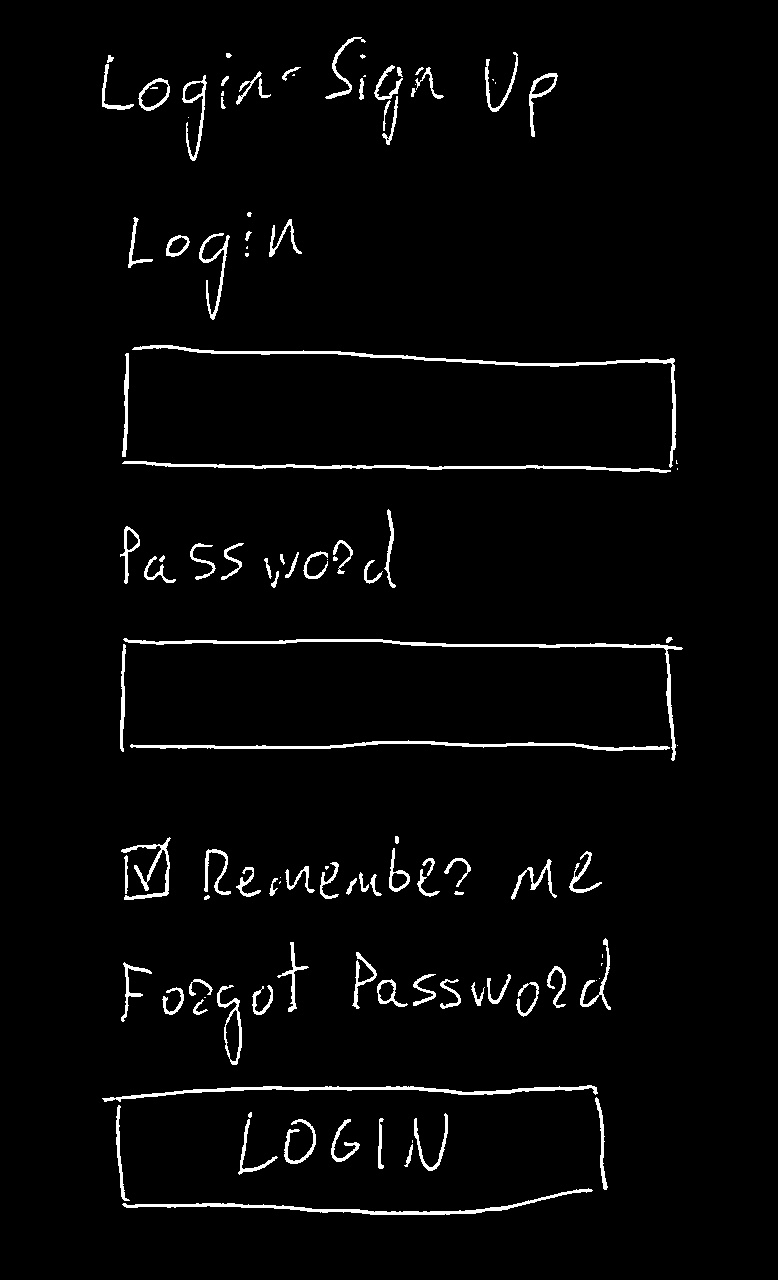
\includegraphics[width=6in]{grayscale.jpg}
      		\caption
      		{Output after grayscale transformation}
      	\end{figure}

      \subsubsection{Adaptive thresholding}
        Further the grayscale image can be reduced to binary image, this helps enhance the strokes of the characters and the figures drawn by the user and eliminates all the fine noise[5] in and around the image. A mean value of pixels in a kernel are calculated this is the threshold value of the kernel, a constant value is subtracted from this and the result is compared with the cutoff number, this generated a binary output which is used to binarize the image. The dimensions of the kernel are 7x7 and a very low cutoff value ~10 is used as the major component of the image is close to white i.e the color of the paper. An inverted binary output is generated.
        \begin{figure}[H]
      		\centering
      		
\includegraphics[width=6in]{adaptive.jpg}
      		\caption
      		{Output after adaptive thresholding transformation}
      	\end{figure}

      \subsubsection{Dilation}
        The image is further dilated iteratively to group the nearby elements in order to avoid fragmented region detection.Dilation is a morphological operation which reduces noise and helps join disparate elements in the image. The primary goal of this step is to merge the nearby contours and hence generate bigger, less fragmented regions. A rectangular kernel is used for dilation as the natural structure of most sketches generated by humans are horizontal in nature. Eg. Words, Letters, Textboxes. Based on the size and the shape of the kernel we can generate regions which are horizontal or vertical merging of the fragmented contours. The iteration count, dimensions and shape of the kernel can be varied to generate different regions of interest.
        \begin{figure}[H]
      		\centering
      		
\includegraphics[width=6in]{dilation.jpg}
      		\caption
      		{Output after dilation transform}
      	\end{figure}

      \subsubsection{Finding bounding rectangles}
        Multiple contours are detected in the dilated images. The contours are filtered based on the area and the dimensions of the contour to weed out possible regions which are very small or thin compared to the dimensions of the image. Bounding rectangles are created around the contours in order to mark the regions of interest. These bounding boxes can now be used to crop the regions of interest which can be passed to the Convolutional Neural Network for labelling. The predictions with the highest confidence score can be used for generating codes.
        \begin{figure}[H]
      		\centering
      		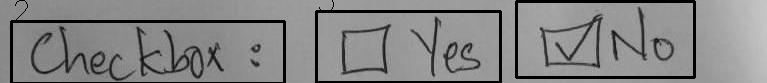
\includegraphics[width=6in]{contour.jpg}
      		\caption
      		{Output after detection of bounding rectangles around regions of interest}
      	\end{figure}

    \subsection{Classification of ROIs}
      Convolutional Neural Networks are widely being used for image classification problems. We used CNN to learn a model by mapping input images to fixed size output vector representing various DOM elements like textbox, radiobutton, checkboxes, labels etc. Now that the Regions of Interests are detected in the previous step they need to be classified into DOM elements. Also there exist some additional falsely detected regions. Such regions need to be discarded.
      \begin{figure}[H]
        \centering
        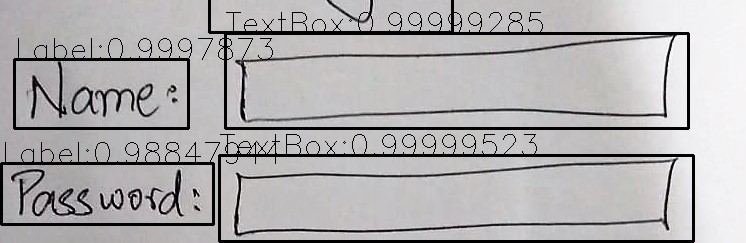
\includegraphics[width=6in]{labelling1.jpg}
        \caption
        {Image classification alongwith confiedence score}
      \end{figure}

      \begin{figure}[H]
        \centering
        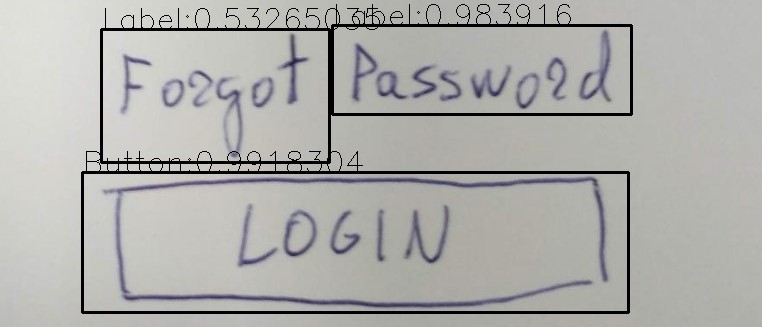
\includegraphics[width=6in]{labelling2.jpg}
        \caption
        {Output from the neural network}
      \end{figure}

      As a part of preprocessing the detected regions were resized into 150x150 images (not maintaining the aspect ratios) and were made grayscale. This input matrix is then passed through two convolution layer and two fully connected layer. The network was kept simple as smaller dataset was available and the problem was simpler. The architecture is shown below:

      \begin{figure}[H]
        \centering
        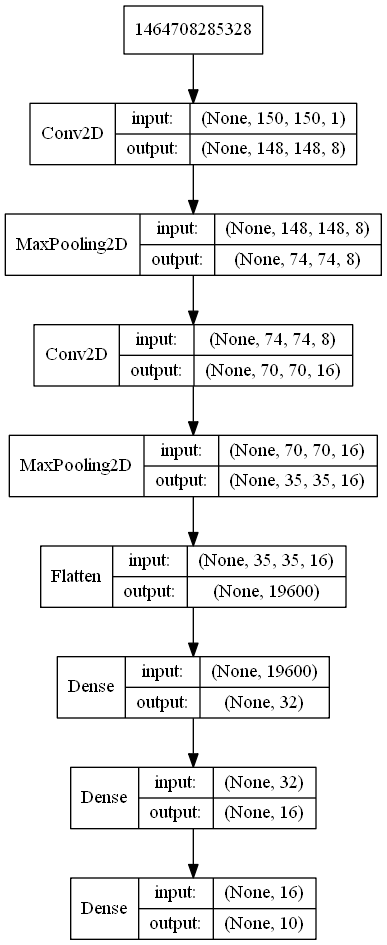
\includegraphics[width=4in]{model}
        \caption
        {The structure of the neural network used for training}
      \end{figure}

      A threshold on the confidence score was set. This helped to discard the falsely identified regions as they did not clear the set threshold.
      The model gave a validation accuracy of around 84% after training it for 75 epochs. The less accuracy was majorly due to confusion between radio buttons, check boxes, labels and headings. There is not much visual dissimilarity between them. There is still scope to increase the accuracy of this model by further experimentation.

      \subsection{ Handwriting Recognition}
        There are many cases where the text is written inside the design components. Some examples are hints in textbox, labels, checkboxes, paragraphs. These texts will be handwritten and need to be recognised accurately.

        \begin{figure}[H]
          \centering
          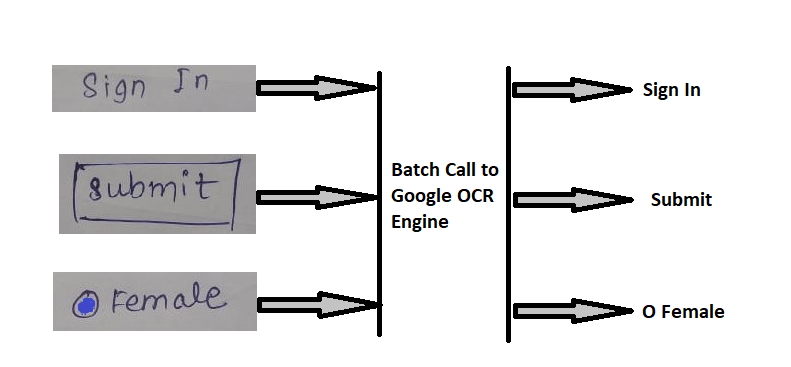
\includegraphics[width=6in]{ocr}
          \caption
          {OCR is performed using Google OCR service}
        \end{figure}

        Each detected design component from the above step was passed to this Text Recognition model to extract the handwritten content. This text will be then associated with the detected component for further steps. Google Optical Character Recognition engine is used as it provides highest handwritten text recognition accuracy. It also provides batch recognition which helps reduce networking delays and cut short the overall processing time.
        The recognised texts are appended to the classification results and saved in a JSON file. This file can be then processed to generate markup language.

      \section{HTML generator}
      The results of the Neural networks are stored in a structured JSON file. Optical character recognition is performed for components containing text. The JSON object generated is a generic object which can be used for generating web elements based on different technologies.The Web engine converts the JSON formatted document layout file into Markup Language Code by detecting the DOM structure based on the coordinates of the regions and their height/width. To represent document layout in JSON, relative position of the element as well as its dimensions are calculated.
      The format of an example DOM element in the JSON file is the following:
      \begin{verbatim}
      {
          "id": "b5e7d988cfdb78bc3be1a9c221a8f744",
          "type": "textbox",
          "height":"100",
          "width":"100",
          "x":"500",
          "y":"400",
         “value”:”Type here”
          "parent": "60c0b53095f81a7bf551b30c93fd20dd",
          "child": “”
      }
      \end{verbatim}
      Modern Browsers support ‘flex-container’ CSS class. This class has some useful built-in features to make web development easier. Vertical and horizontal stacking of elements can be done by just toggling the value of ‘flex-direction’ attribute of this class.
      Besides all the dimension and type related information about the nodes, document metadata also stored in the JSON (eg. Height, Width). Dependant information is calculated geometrically. Orientation and layout [7] of the tags of the HTML document is decided from document height and width values available in the metadata and corresponding changes are reflected in the flexbox orientation. Web engine converts this document layout JSON into code.

      \section{End to End Experience}
        A web service based on MEAN stack was developed to provide a polished end to end solutions for users to consume the service. Users can upload the images for sketch drawn and the service will process the uploaded image using our custom trained tensorflow model on the server and process the results via the web engine and generate HTML code for the user. The structured JSON file along with the bootstrapped HTML code will be available for download as a compressed object.
        \subsection{Putting it all together}
          The complete application has a modular structure and every logical step can be executed as a standalone process. This has helped accelerate development process and made the application pluggable and hence easily extensible. But for a end user the process has to be simplified and all the different modules should be connected and pass information to each other. The project consists of a NodeJS web server based on express framework which hosts the  project and provides an easy to access web interface to the web user. The server also has TensorFlow installation along with our custom trained modules for image recognition and labelling. This server can be deployed to any machine with almost no prerequisites and makes deployment easy.
          \begin{figure}
            \centering
            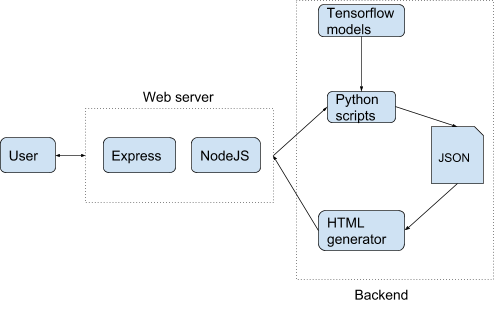
\includegraphics[width=6in]{node}
            \caption
            {Architecture of the Node web service}
          \end{figure}
        \subsection{Process Flow}
          \begin{enumerate}
            \item The user sketches his ideas about the web page and captures it as an image
            \begin{figure}[H]
              \centering
              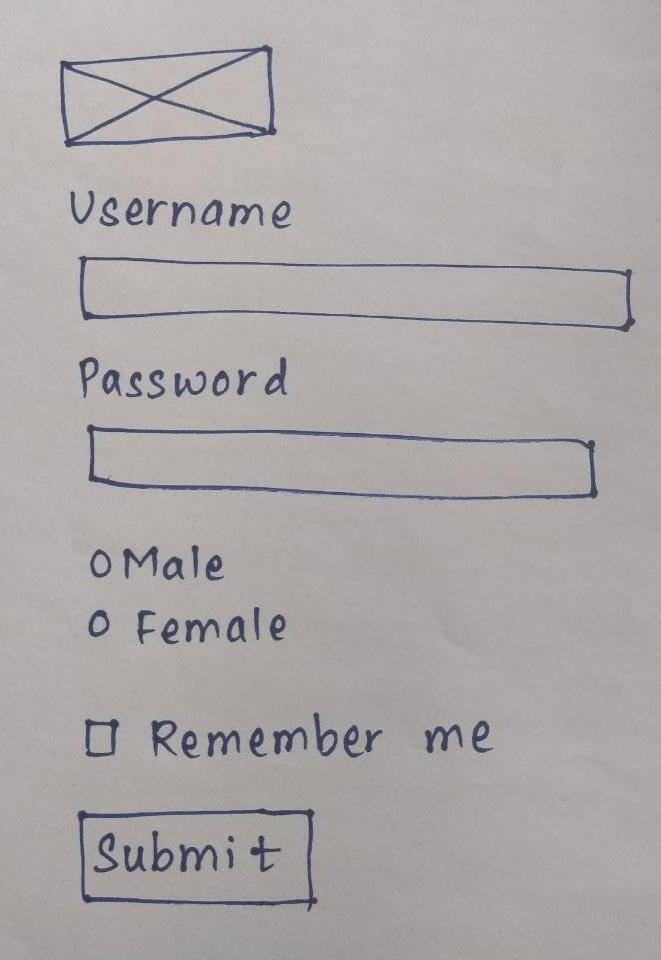
\includegraphics[width=6in]{process1.jpg}
              \caption
              {Sample image of a web mockup drawn on paper}
            \end{figure}
            \item The images are uploaded to our web service using any web browser
            \begin{figure}[H]
              \centering
              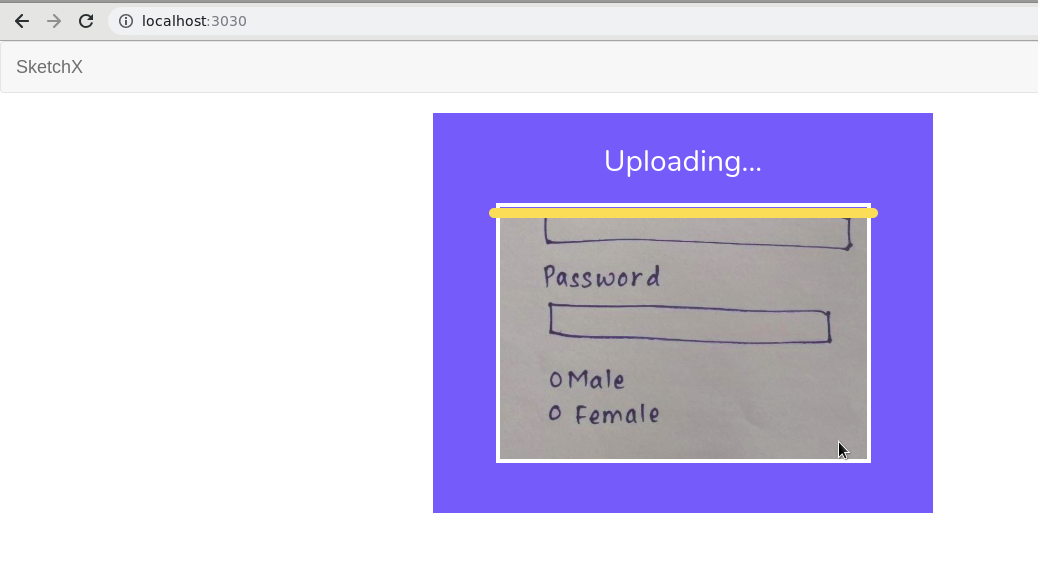
\includegraphics[width=6in]{process2}
              \caption
              {Snapshot of the web service while uploading an image}
            \end{figure}
            \item The backend processes the images and generates HTML code along with metadata
            \item The user can preview the generated code and download the code for further development
            \begin{figure}[H]
              \centering
              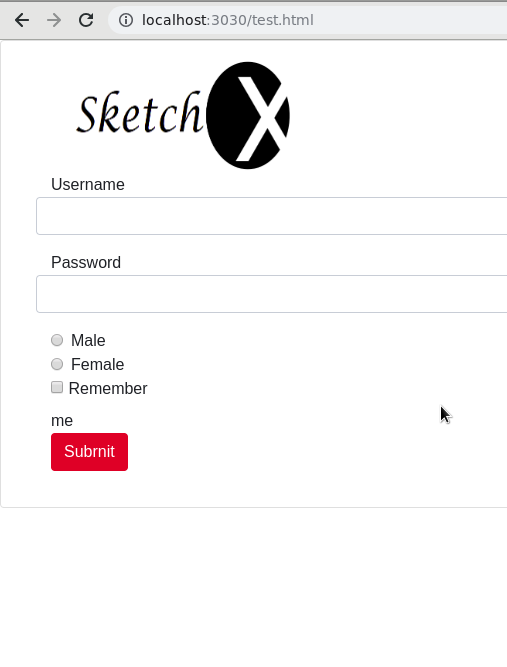
\includegraphics[width=6in]{process3}
              \caption
              {Preview of the HTML code generated by the service}
            \end{figure}
          \end{enumerate}


%_____________________________________________________________________________________________
